\chapter{Master Control Program}
\label{appendiceD}
\thispagestyle{empty}
\noindent Apart from the two telescpes described in Appendix C, the Helios solar observatory is composed by a dome, a mount, a weather station and two camera sensors (one for each telescope). Here are the specifications:
\begin{itemize}
  \item a Scopedome 3M dome;
  \item a Celestron CGEM mount;
  \item a AAG CloudWatcher weather station.
  \item two 2 QHY5-II-M planetary cameras with a 1/2 CMOS sensor;
\end{itemize}
All these components come with dedicated proprietary software programs to control them. The problem with these programs is that, apart from some predefined functionality, they are not able to work together. Therefore, in order to fully automate the observatoy, it was necessary to build a dedicated control program.
\bigbreak
\noindent All the hardware was selected according to its capability of being programmed. The protocol that was used in order for the master control program to interface with the hardware is called ASCOM (Astronomy Common Object Model). ASCOM establishes a set of vendor, language and platform independen interface standards for drivers that provide plug-and-play control of astronomical instruments and related devices.
\bigbreak
\noindent The master control program is a very large project, that I started during 2018 and is still ongoing. During my internship I was able to program the connection to the components and a part of the user interface that lets the operator control the observatory manually. For what concerns the automation of the daily observation process, I focused on the improvement of the tracking of Sun.
\bigbreak
\noindent Some tracking capabilities were already offered by the Celestron mount. In fact, once the telescope has slewed to some coordinates, it is able to follow that particular point in the sky, regardless of the rotation of the Earth. This functionality is called tracking, and it is included in any modern mount. The telescope moves thanks to a set of motors and gears that are embedded inside the robotic arm. Like any mechanism, it has imperfections and tolerances, that make the accuracy of the tracking is bounded.
\bigbreak
\begin{figure}[t!]
    \centering
    \captionsetup{justification=centering}
    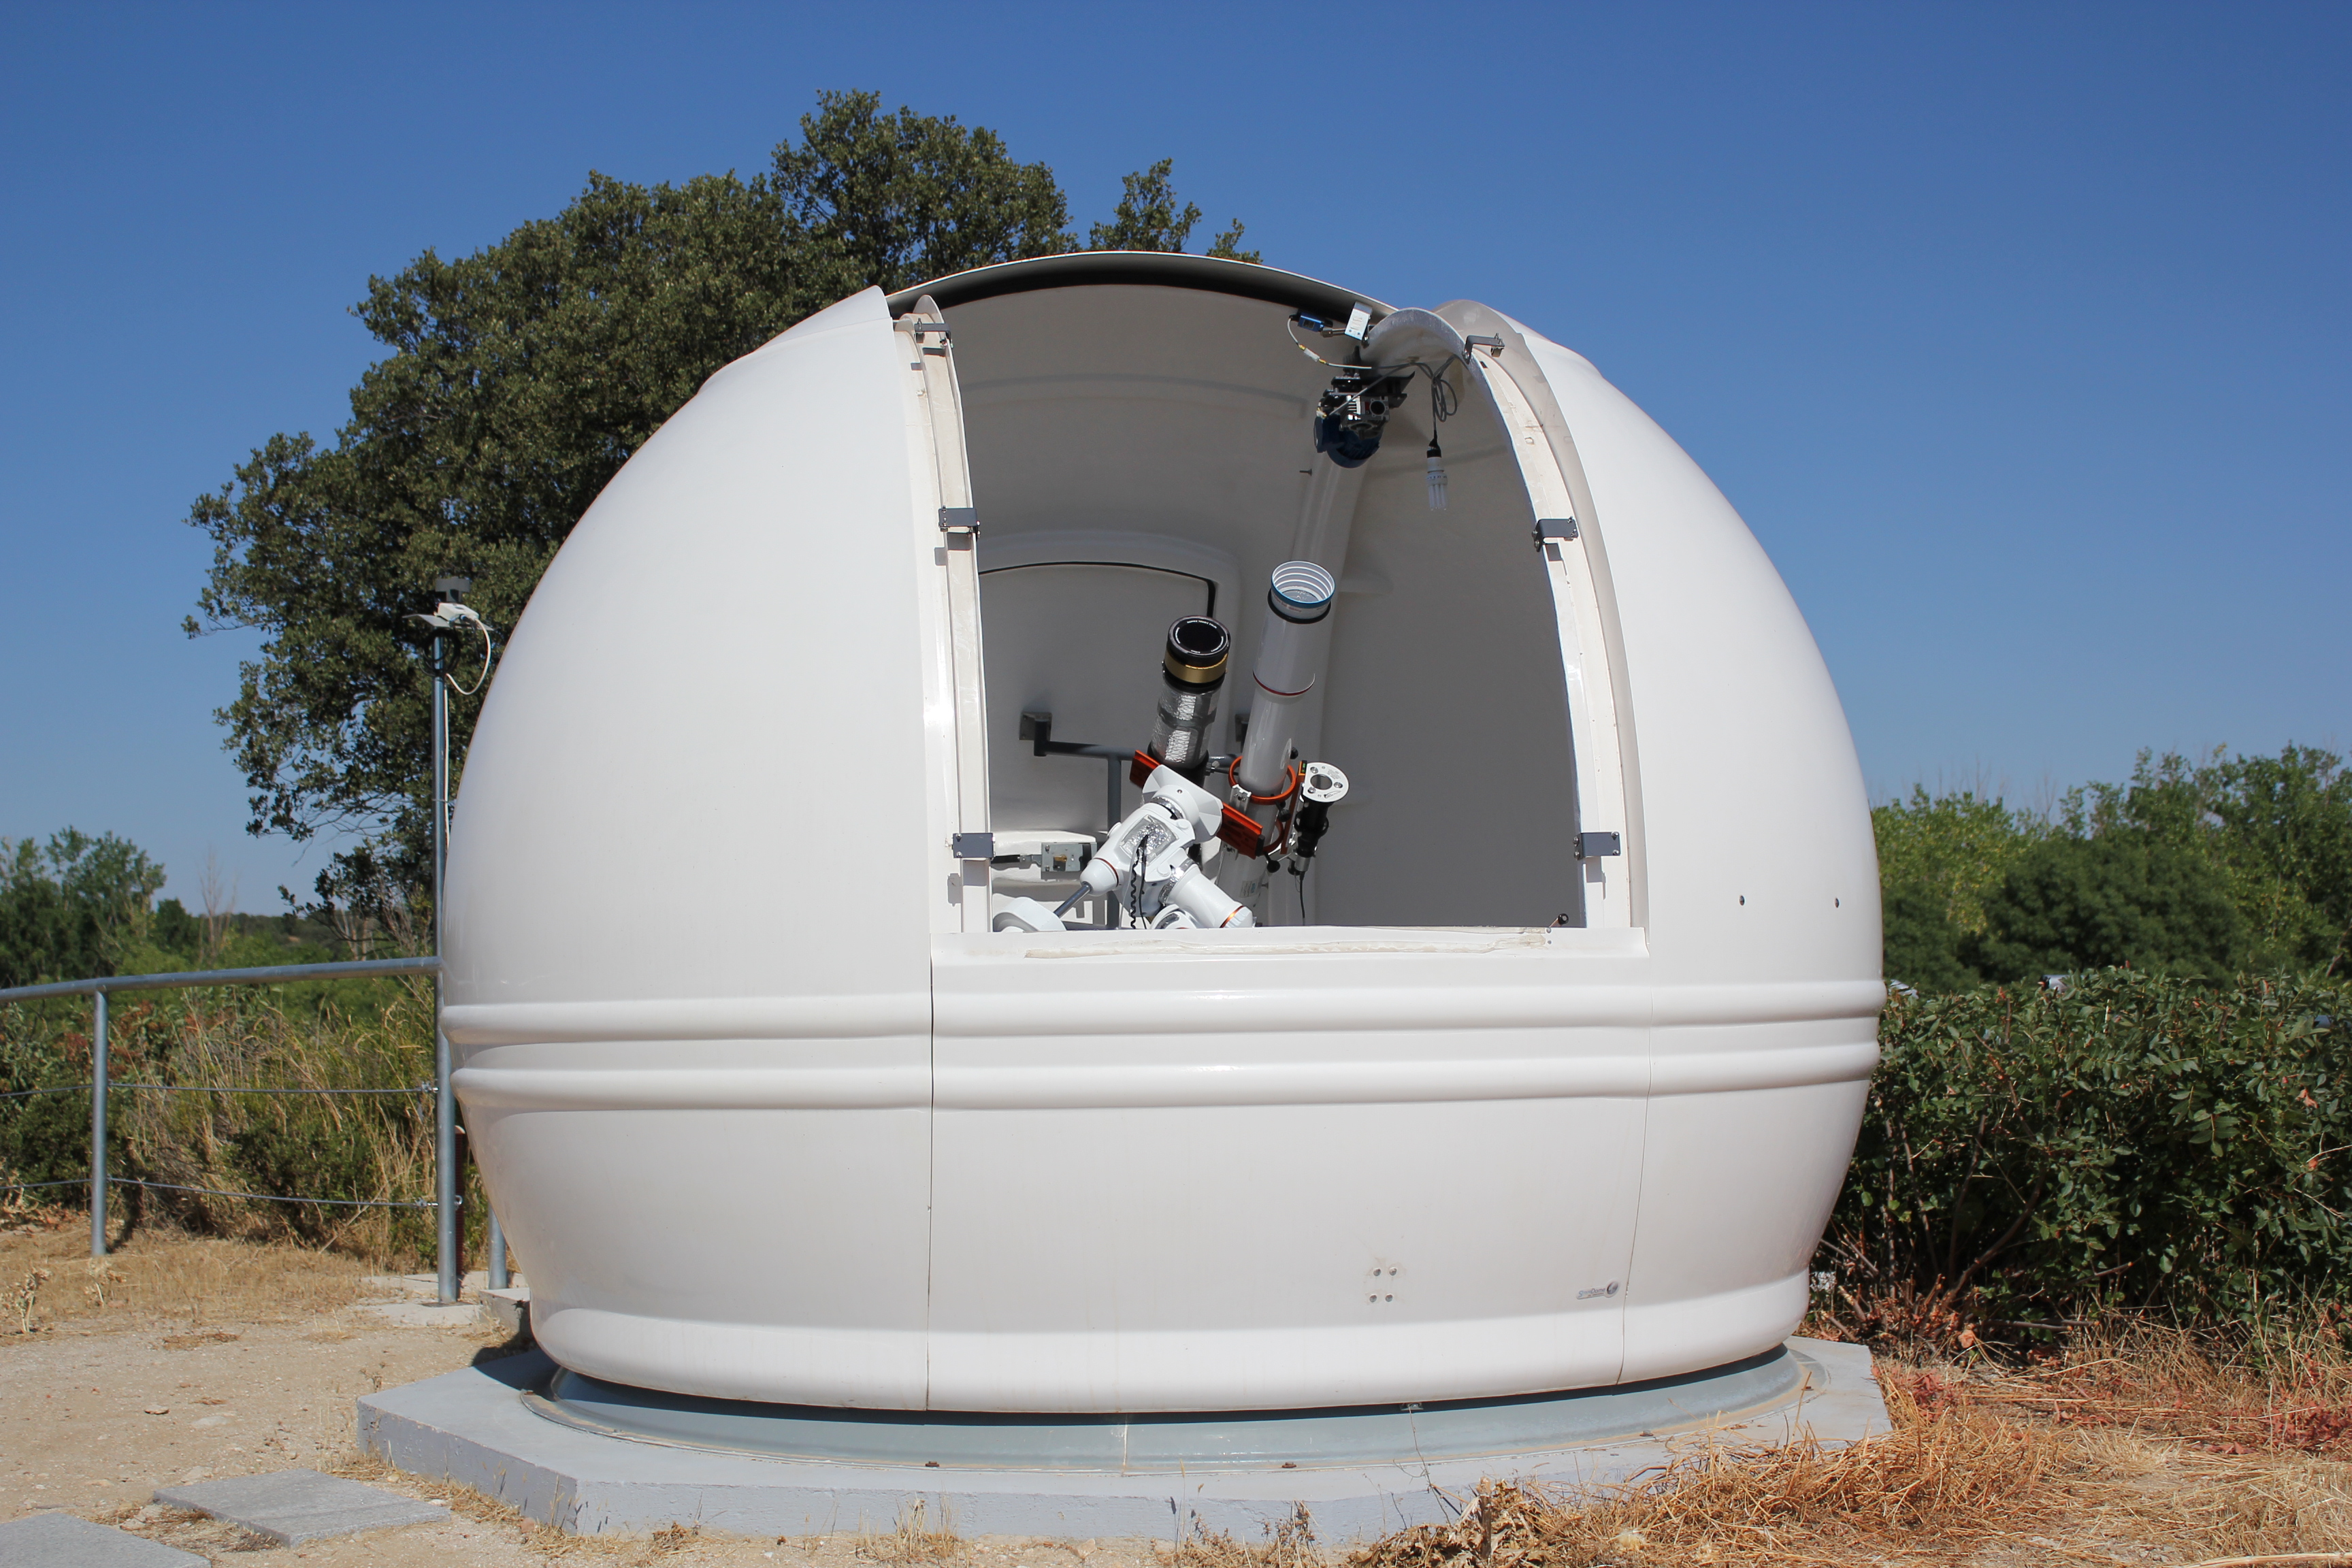
\includegraphics[width=\textwidth]{./pictures/helios}
    \caption{An image of the Helios observatory performing daily observation}
    \label{fig:halpha-visible}
\end{figure}
\noindent The limitations of the mechanical tracking resulted in misalignments in the images, and in some cases in the Sun ending out of the field of view. To address this problem software can come to the aid of hardware. In fact, the two camera sensors stream images in real time from the scope to the control program. As shown in Appendix C, it is fairly easy to find the coordinates of the center of the disk. Hence, it is also possible to calculate the correction that should be applied by the mount to place it back to the center of the frame. In fact, using the same reasoning as in \eqref{eq:radpix}, we can compute how many radians correspond to each pixel of the image and, after some coordinate translation, instruct the telescope to slew back to the Sun.
\bigbreak
\noindent The development of the master control program for is being continued by the interns that followed me at the Helios observatory.
